\documentclass[11pt,dvipdfmx,a4paper]{jsarticle}

\usepackage{amsmath,amssymb}
\usepackage{bm}
\usepackage[dvipdfmx]{graphicx}
\usepackage{physics} % http://mirrors.ibiblio.org/CTAN/macros/latex/contrib/physics/physics.pdf
\usepackage{siunitx} %SI単位を楽に出力
\usepackage{mathtools} %環境の追加
% \usepackage{circuitikz} %電気回路をtex中で書く
% \usepackage{caption} %番号なしキャプションを書く
% \usepackage{cancel} %式中に斜線を入れる
% \usepackage{tensor} %テンソルの添え字を書く
% \usepackage{tikz} %図を書く
% \usepackage{ascmac} %四角い枠の中に文章を書く
% \usepackage{float} %figureで[hbp]オプションを使う
% \usepackage{hyperref}  \usepackage{pxjahyper} %ハイパーリンクをつかう
% \usepackage{tablefootnote} %表中に注釈をいれる
% \usepackage[thicklines]{cancel} %数式中の取り消し線
\usepackage[version=4]{mhchem} %化学式の入力
\usepackage{pdfpages}
% \usepackage{wrapfig} %文章の回り込み
\usepackage[subrefformat=parens]{subcaption} %(a)図のようにすることができるやつ
\usepackage{here}
\usepackage{mathrsfs} % TODO テンプレートに追加
\usepackage{url} % TODO テンプレートに追加
\usepackage[margin=15mm]{geometry} %余白の削除

\graphicspath{{./image/}}

\begin{document}

%出力したpdfを表紙にするとき
% \includepdf[pages=1,noautoscale=false]{cover.pdf}
% \newpage

%texで表紙を書くとき
\quad\\[35mm]
\centerline{\Huge{\textsf{第 4 回}}}
\quad\\[5mm]
\centerline{\Huge{\textsf{応 用 物 理 学 実 験}}}
\quad\\[5mm]
\begin{table}[h]
	\centering
	\begin{tabular}{| c | c |}
		\hline
		\Huge\textsf{{題目}} & \Huge{\textsf{電気伝導度の温度依存性}} \rule[-5mm]{0mm}{15mm} \\
		\hline
	\end{tabular}
\end{table}
\quad\\[10mm]
\begin{table}[h]
	\centering
	\begin{tabular}{l l}
		\hline
		\LARGE{\textsf{氏\qquad 名}} & \LARGE{\textsf{: 西原 翔}} \rule[0mm]{0mm}{6mm} \\
		\hline
		\LARGE{\textsf{学  籍  番  号}} & \LARGE{\textsf{: 1522068}} \rule[0mm]{0mm}{6mm} \\
		\LARGE{\textsf{学部学科学年}} & \LARGE{\textsf{: 理学部第一部応用物理学科3年}}\\
		\hline
	\end{tabular}
\end{table}
\quad\\[10mm]
\centerline{\LARGE{\textsf{共同実験者:1522064 中井空弥}}}\\[2mm]
\centerline{\LARGE{\textsf{\qquad\qquad\quad\;\;1522091 宮田祟杜}}}\\[2mm]
\centerline{\LARGE{\textsf{\qquad\qquad\quad\;\;1522095 村山涼矢}}}\\[2mm]
\centerline{\LARGE{\textsf{\qquad\qquad\quad\;\;1522B02 中村洸太}}}\\[2mm]
\quad\\[10mm]
\centerline{\LARGE{\textsf{提出年月日:2024年06月27日}}}\\[2mm]
\centerline{\LARGE{\textsf{実験実施日:2024年06月14日}}}\\[2mm]
\centerline{\LARGE{\textsf{\qquad\qquad\quad\;2024年06月21日}}}
\quad\\[10mm]
\centerline{\LARGE{\textsf{東 京 理 科 大 学 理 学 部 第 1 部}}}\\[2mm]
\centerline{\LARGE{\textsf{応 用 物 理 学 教 室}}}

\thispagestyle{empty}
\clearpage
\addtocounter{page}{-1}
\newpage

% \twocolumn
\section{目的}

\section{原理}
\subsection{ドルーデモデル}
量子論以前の1900年頃、
ドルーデは電気伝導について古典的なモデルを立てて議論した。
電子を外部電場\(\mathscr{E}\)のなかの理想気体と考え、
古典的な運動方程式で記述する。
電子気体はイオンや欠陥によって散乱されるものとして、
運動方程式を立てると。
\begin{align}
    m\dot{v} + \frac{m}{\tau}v = -e\mathscr{E} % \tag{9.42}
\end{align}
このときの\(v_D\)はドリフト速度というもので電子の速度から
電場のない熱平衡状態における電子の速度\(v_{\text{therm}}\)
を用いて
\begin{align}
    v_D= v-v_{\text{therm}}
\end{align}
と表されるものである。
電場がないときこの古典的な運動方程式の解としては
\begin{align}
    v = v_{\text{therm}}\qty(1-e^{-t/\tau})
\end{align}
である。
電場があるときには解は
\begin{align}
    v = -\frac{e\mathscr{E}\tau}{m}\qty(1-\exp\frac{-t}{\tau})
\end{align}
となっているので\(\tau\)は平衡状態に達するまでの緩和時間。
ドリフト速度は
\begin{align}
    v_D=-\frac{e\tau}{m}\mathscr{E} % \tag{9.43}
\end{align}
となる。
これより電場方向の電流密度は熱平衡状態では電流が流れてないのでドリフト速度を用いて
\begin{align}
    j = -env_D = ne\mu\mathscr{E} = \frac{e^2\tau n}{m}\mathscr{E} % \tag{9.44}
\end{align}
このとき\(n\)は自由電子の体積密度、
移動度\(\mu\)は電場をかけたときのドリフト速度の比例定数。
これより伝導度は
\begin{align}
    \sigma = \frac{j}{\mathscr{E}} = \frac{e^2n\tau}{m} % \tag{9.45}
\end{align}
と表される。
この式より、電気伝導度は電流のキャリア濃度に比例することがわかる。

\subsection{半導体への不純物ドーピング}
半導体に電子をドープしたときのバンドの様子を考える。
バンドモデルでは一電子近似の元で考える。
周期ポテンシャルのもとのシュレーディンガー方程式は
周期ポテンシャルを \(V(r)\), ドープした原子によるポテンシャルを \(\hat{H}'(r)\) として
\begin{equation}
	\qty(-\frac{\hat{p}^2}{2m}+V+H')\psi = E \psi
\end{equation}
となる。
\(H'(r)\) によるポテンシャル変化は周期ポテンシャルに比べ変化はゆっくりしている。
こうしたときには周期ポテンシャルによる波動関数への寄与は質量の部分に取り込むことができる。
今回使う半導体は \ce{n-Ge} であり伝導体の最下部は \(\Gamma\) 点にある。

なので
\begin{equation}
	\qty(-\frac{\hbar^2}{2m^*}+\hat{H}'(r))F() = (E-E_c)F(r)
\end{equation}
とできる。ドープした原子は陽イオンとみなせるため
\begin{equation}
	\hat{H}'(r) = -\frac{e^2}{4\pi\varepsilon r}
\end{equation}
とできる。するとこれは水素原子と同じ問題になるため、この固有値方程式の固有値は
\begin{equation}
	E-E_c = -\frac{m^*}{2}\qty(\frac{e^2}{4\pi\varepsilon})\frac{1}{n^2}
\end{equation}


\subsection{四端子法}

\section{実験}
金属、p 型半導体、超伝導体の電気伝導度の温度依存性を調べるため、
金属として \ce{Pt}, p 型半導体として \ce{n-Ge}, 超伝導体として \ce{Nb} を試料とし、
断熱して温度を下げやすくするため、真空中に端子づけした試料をいれ、
四端子法と二端子法にて185 K から \ce{Nb} が超伝導相へと相転移する 8 K 程度まて
電気伝導度を測定した。その際に使った真空ポンプの様子は図\ref{pic:measure_system}

この系の電気回路は図\ref{fig:circuit_system}の通りになっている。

\begin{figure}[h]
	\centering
	% 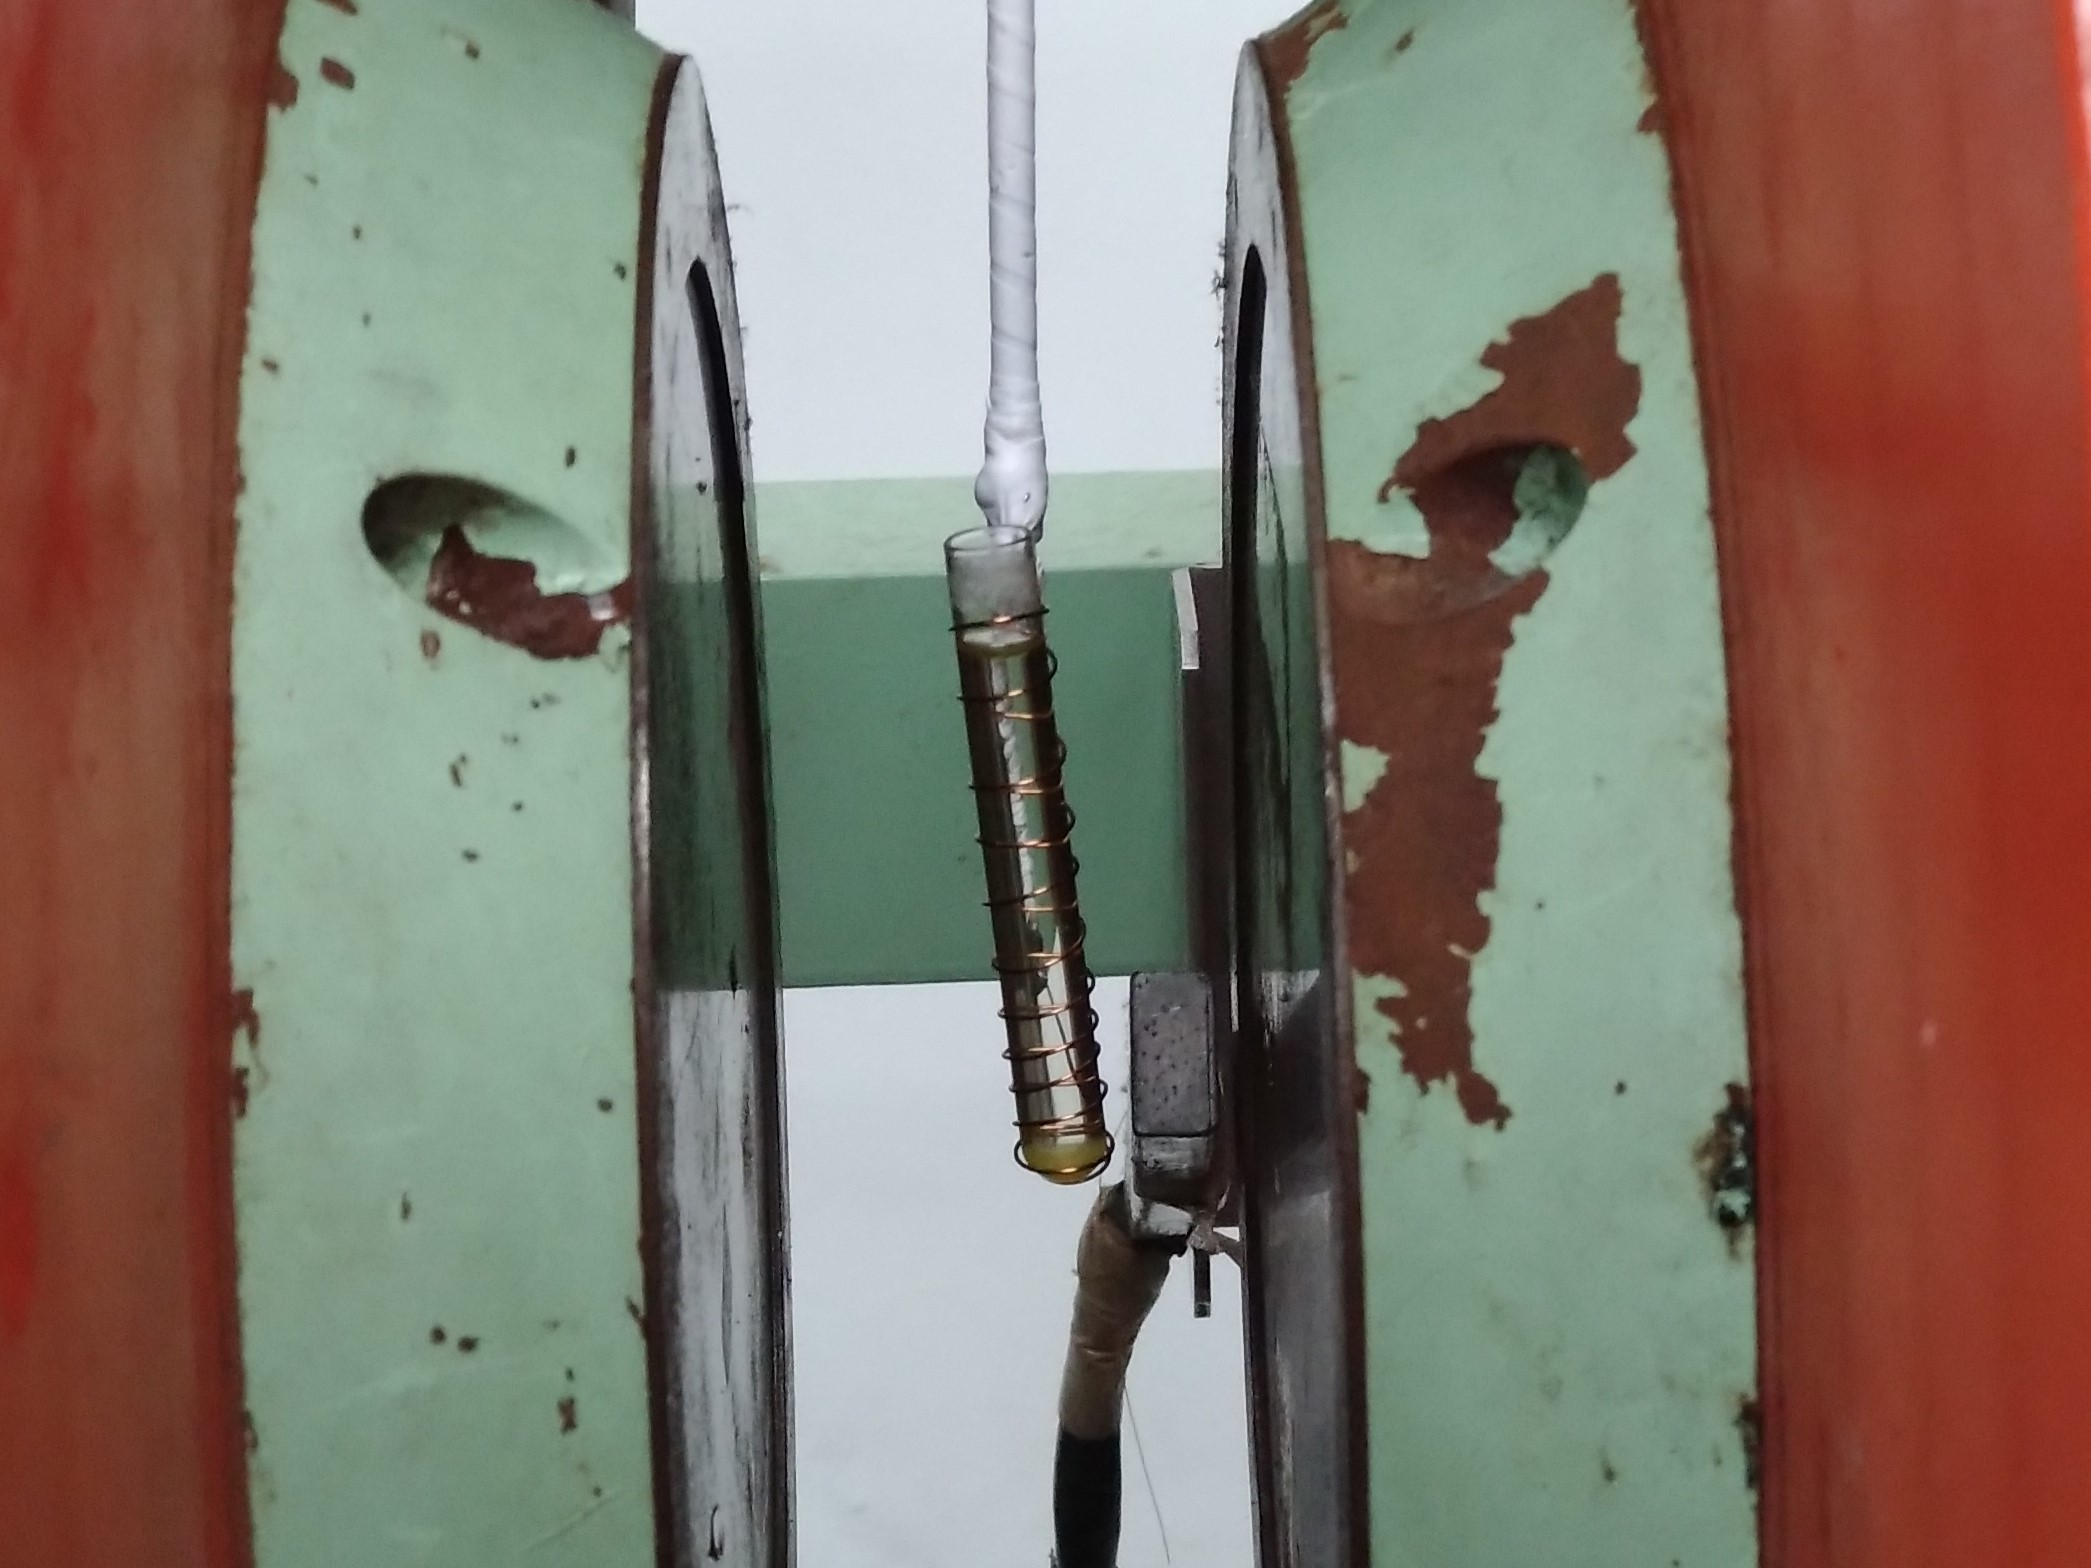
\includegraphics[width=0.5\columnwidth]{pic/01.JPG}
	\caption{
		電気伝導度を真空中で測定する装置。
		上部から出ている管は試料室の温度を下げるための冷媒が流れている。
		下部には今回測定する 3 つの試料、\ce{Pt}, \ce{n-Ge}, \ce{Nb} が端子づけされた状態で入っている。
		左には真空へと排気するポンプへつながる管がつながっている。
	}
	\label{pic:measure_system}
\end{figure}

\section{結果}
\ce{n-Ge} の電気伝導度を二端子法と四端子法で測定した結果をアレニウスプロットする図\ref{graph:n-Ge_ex}のようになった。



\section{考察}

\section{結論}


\bibliographystyle{junsrt}
\bibliography{reference}
% グリュナイゼンの論文

\section*{付録}
今回の実験に関係する理論を教科書\cite{ibach-luth}を使って学んだときのノートを付録に追記する。
\section{金属の電気伝導度}



\subsection{ボルツマン方程式による電気伝導度の導出}
% 9.2 節でホールを扱ったがここでやったのと同じように
量子・古典対応を使いながら考えてみる。
粒子流密度は第一ブリューアンゾーンでの積分を用いて
\begin{align}
    j_n = \frac{2}{(2\pi)^3}\int_{\text{1stBZ}} v(k)f(k) d^3k % \tag{9.47}
\end{align}
電場がそこまで強くないとき分布関数は
\begin{align}
    f(k) = f_0(k) + \frac{e}{\hbar}\tau(k)\mathscr{E}\cdot\nabla_kf_0(k)
\end{align}
となるので電場の向きを\(x\)軸とすると、電流密度\(j\)は
\begin{align}
    j = -ej_n = -\frac{e}{4\pi^3} \int d^3k\,v(k) \qty(f_0(k)
    +\frac{e\tau(k)}{\hbar}\mathscr{E}_x\pdv{f_0}{k_x}) % \tag{9.48}
\end{align}
平衡状態では\(v(k)f_0(k)\)の積分は対称性から消え、残りの部分は
\begin{align}
    \pdv{k_x} = \pdv{E}{k_x}\pdv{E} = \hbar v_x \pdv{E} % \tag{9.50}
\end{align}
なので
\begin{align}
    j &= -\frac{e^2}{4\pi^3}\mathscr{E}_x\int dk^3 v_x^2(k)\tau(k)\pdv{f_0}{E} \\% \tag{9.52}\\
    \sigma &= \frac{j}{\mathscr{E}_x} = -\frac{e^2}{4\pi^3}\int dk^3 v_x^2(k)\tau(k)\pdv{f_0}{E} % \tag{9.52}\\
\end{align}
平衡状態におけるフェルミ分布関数を考えると
傾きがあるのはエネルギーがフェルミ準位付近しかなく、
その傾きは \(-1/4k_BT\)程度である。
\begin{align}
    \pdv{E}\,f_0(E_F,T) &= \pdv{E}\qty[\frac{1}{e^{(E-E_f)/k_BT}+1}]_{E=E_F}\\
    &=\qty[-\frac{e^{(E-E_f)/k_BT}/k_BT}{\qty(e^{(E-E_f)/k_BT}+1)^2}]_{E=E_F}\\
    &=\frac{1}{4k_BT}
\end{align}
なので
\begin{align}
    \pdv{f_0}{E} \sim -\frac{1}{4k_BT}\delta(E-E_F)
\end{align}
という風に近似しそうだがもっと近似して
\begin{align}
    \pdv{f_0}{E} \sim -\delta(E-E_F) % \tag{9.53}
\end{align}
というようにする。\footnote{自明とか言ってるけど温度無視していいのかしら?}\\
また角波数空間の積分を同じエネルギーを持つ面の面素\(df_E\)と
それに垂直な方向\(dk_{\perp}\)に分けると
\begin{align}
    d^3k =df_Edk_\perp = df_E \frac{dE}{|\nabla_k E|} = df_E \frac{dE}{\hbar v(k)} % \tag{9.54}
\end{align}
なので
\begin{align}
    \sigma &= -\frac{e^2}{4\pi^3}\int dk^3 v_x^2(k)\tau(k)\pdv{f_0}{E} \\% \tag{9.52}\\
    &=\frac{e^2}{4\pi^3\hbar}\int df_E \, dE \frac{v_x^2(k)}{v(k)}\tau{k}\delta(E-E_F) \\% \tag{9.55}\\
    &=\frac{e^2}{4\pi^3\hbar}\int_{E=E_F}\frac{v_x^2(k)}{v(k)}\tau(k) df_E \\% \tag{9.56}
\end{align}
となる。
この積分がどのようなものか少し考える。
積分の中身の期待値を考え積分の外側に出してみる。
速度については
\begin{align}
    v^2(k) = v_x^2(k) + v_y^2(k) + v_z^2(k) = 3 v_x^2\\
    \frac{v_x^2}{v} = \frac{v^2(k)}{3v(k)}
\end{align}
と考えられるので
\begin{align}
    \sigma = \frac{e^2}{4\pi^3\hbar}\times \frac{v(k_F)\ev{\tau}}{3}\int_{E=E_F} df_E
\end{align}
残ったフェルミ面の面積を考える。
フェルミ波数は古典・量子対応関係より運動量を考えて
\begin{align}
    m^*v(E_F) = \hbar k_F % \tag{9.57a}
\end{align}
の関係がある。
ほとんど自由な電子ではフェルミ面は球になっていて、また\(k_BT <<E_F\)になっているので
また体積当たりの電子の数はフェルミ球の体積を\((2\pi)^3\)で割ったものとなる。
つまり
\begin{align}
    n = \frac{2 \times 4 \pi k_F^3/3}{(2\pi)^3} \qquad \leftrightarrow \qquad
    k_F^3 = 3\pi^2n % \tag{9.57c}
\end{align}
となっている。\footnote{スピン自由度のせいで体積がは2倍になっている。}
では表面積は
\begin{align}
    \int_{E=E_F} df_E &= 4\pi k_F^2\\ % \tag{9.57b}\\
    &=\frac{12\pi^3n}{m^*v(E_F)/\hbar}
\end{align}
となる。\footnote{スピン自由度のせいで表面積は2倍になっていると思いきやフェルミ面の"表面積"を考えてるのでいらない。}
よって
\begin{align}
    \sigma &= \frac{e^2}{4\pi^3\hbar}\times \frac{\ev{v}\ev{\tau}}{3}\int_{E=E_F} df_E\\
    &=\frac{e^2\ev{\tau}}{12\pi^3\hbar} v(k_F) \times\frac{24\pi^3n}{m^*v(E_F)/\hbar}\\
    &=\frac{e^2n\ev{\tau}}{m^*}
\end{align}
という風にドルーデモデルで得られた伝導度と同じようになる。

ドルーデモデルがなぜうまくいくのかの説明として伝導度と移動度が一致しているからとある。
これだけだと説明になってない気がするが、おそらくうまいこと非平衡なフェルミ分布関数の積分を取り入れられてるからなのだろう。
もっと考察できそうだが\dots

\subsection{電気伝導度と温度の関係}
電気伝導度の温度変化を考えるには\(\tau(E_F)\)の温度変化を考えればよい。
というのもキャリアの密度\(n\)は
\begin{align}
    n = \frac{2\times 4\pi k_F^3 /3}{(2\pi)^3} % \tag{9.57c}
\end{align}
の式を見ると、変数はフェルミ波数つまりフェルミエネルギーだけによるので温度によらないと考えられる。

\(\tau\)を厳密に量子力学による計算に代わりにフォノン、不純物などの欠陥による散乱の効果を定性的に議論する。
フォノン散乱、欠陥による散乱は別々のメカニズムであるから
全散乱確率は両者の散乱確率の和となる。
緩和時間というのは一回散乱するまでの時間と考えられるので散乱する確率はそれの逆数となる。
\begin{align}
    \frac{1}{\tau} = \frac{1}{\tau_{ph}} +\frac{1}{\tau_{def}} % \tag{9.59}
\end{align}
ph は phonon, def は defect の略。

この取り扱いの右辺の各項の性質を考えると電気伝導度が出る。
まず、単位時間当たりの衝突回数は散乱断面積\(\Sigma\)と粒子測度の積に比例する。
\footnote{ぶつかる面が大きかったら当たりやすいし、速度が速かったらいっぱい動き回るので衝突回数も増える。}
\begin{align}
    \frac{1}{\tau} \propto \Sigma v
\end{align}
金属の伝導電子に関しては\(v\)はフェルミ面付近の電子なのでフェルミ速度\(v(E_F)\)に他ならず、温度によらない。

散乱中心が欠陥の場合には散乱断面積\(\Sigma\)も温度によらない。
\footnote{そうなの?}
つまり欠陥による電気伝導度は温度によらない。

フォノン散乱による場合は波数ベクトル\(q\)各振動数\(\omega_q\)のフォノンの振幅の2乗平均
\(\ev{s^2(q)}\)に比例し、\footnote{見つからない\dots}
十分高温のとき、エネルギー等分配則から
\begin{align}
    M\omega_q^2\ev{s^2(q)} = k_BT % \tag{9.60}
\end{align}
ここで\(M\)はイオン核の質量で電子質量よりも重いため?
\begin{align}
    \frac{1}{\tau_{ph}}\propto \ev{s^2(q)}\propto \frac{k_BT}{M\omega_q^2} % \tag{9.61a}
\end{align}
フォノン振動数だとイメージしにくいので見積もりのため、\(\omega_q\)デバイ振動数として
これをデバイ温度に読み替えたものを考える。
\begin{align}
    \hbar \omega_D = k_B \Theta
\end{align}
より
\begin{align}
    \tau_{ph} \propto \frac{M\Theta^2}{T} % \tag{9.61b}
\end{align}

よってデバイ温度以上の高温では電気抵抗率\(\varrho=1/\sigma\)は
\begin{align}
    \rho = \frac{1}{\sigma} = \frac{m^*}{e^2n} \frac{1}{\tau}
    = \frac{m^*}{e^2n} \qty(\frac{1}{\tau_{def}} + A\frac{T}{M\Theta^2})
\end{align}
となり電気抵抗率は温度は比例する。(マティーセンの規則)

低温でグリュナイゼン(1933)は
\footnote{ドイツ語の原論文(\url{https://sci-hub.hkvisa.net/10.1002/andp.19334080504})
どうやって式を出したかわからないし、ぱっと見同じ式には見えない。この中で引用されている E. Gruneisen, Leipziger Vortrage 1930 にあるのかもしれない。
しかしこれが見つからない。}
\begin{align}
    \varrho_{ph}=A\qty(\frac{T}{\Theta})^5\int_0^{\Theta/T} \frac{x^5dx}{(e^x-1)(1-e^{-x})} % \tag{9.62}
\end{align}
この式を用いていろんな金属の電気抵抗率の測定値と比較してうまくいったことを言ってる。
つまり
\begin{align}
    \varrho_{ph}(T) \propto T^5
\end{align}
% \begin{figure}[h]
%     \centering
%     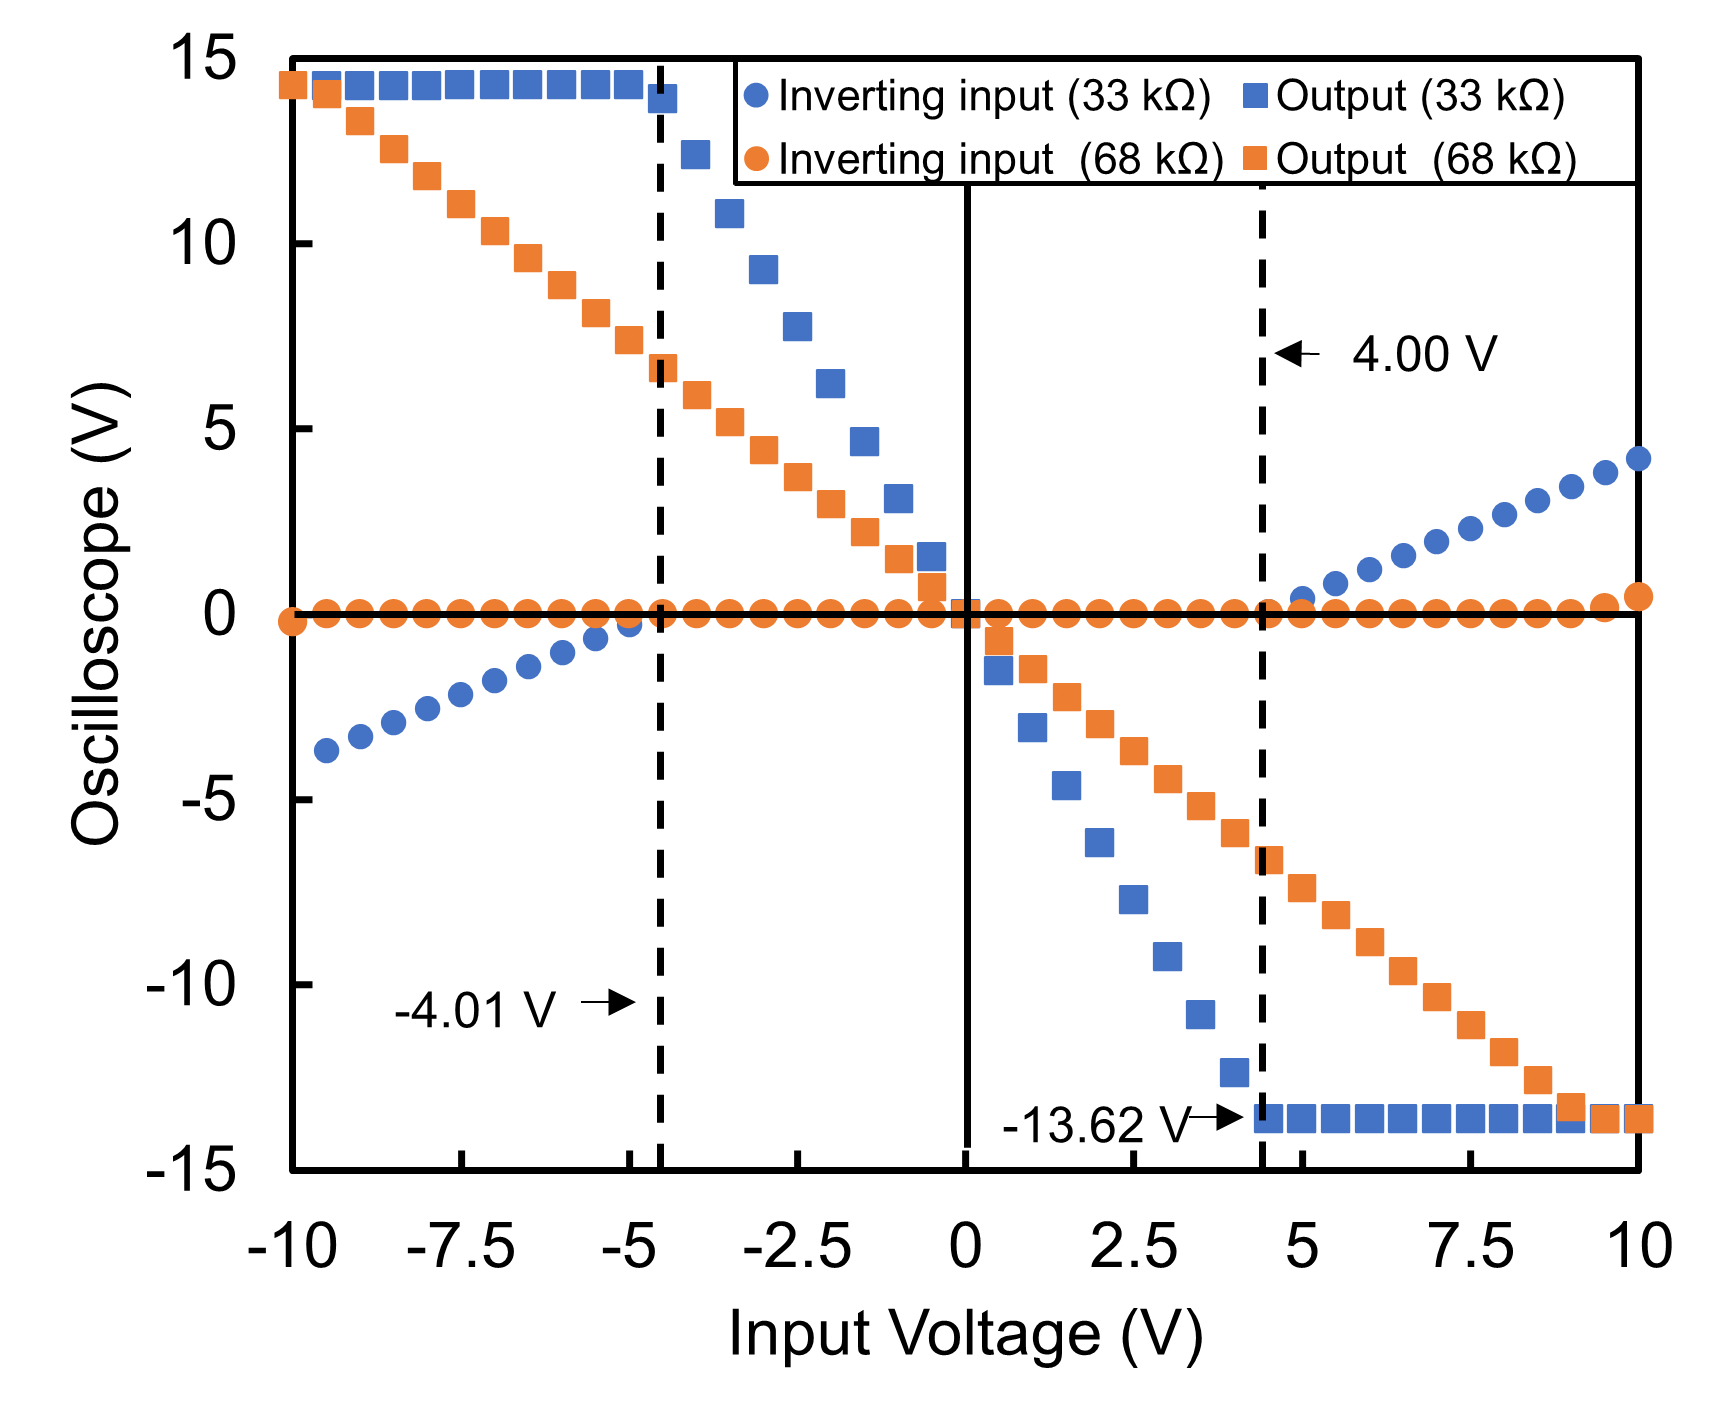
\includegraphics[width=0.94\columnwidth]{fig1.JPG}
% \end{figure}

\section{熱電効果}
\subsection{温度勾配と電流密度}
電気伝導度を導出するときの近似をゆるめて考える。
分布関数が位置に依存すると考える。
\begin{align}
    f(k) = f_0(k) + \frac{e}{\hbar} \tau\mathscr{E} \cdot \nabla_k f - \tau v \cdot \nabla_r f % \tag{9.64}
\end{align}
そして
\begin{align}
    \nabla_r f(k,\, T(r)) = \pdv{f}{T} \nabla_r T
\end{align}
なので摂動が小さいときを考えて
\begin{align}
    f(k) = f_0(k) + \frac{e}{\hbar} \mathscr{E} \cdot \nabla_k f - \tau \pdv{f_0}{T} v \cdot \nabla_r T % \tag{9.65}
\end{align}
なので電流密度は
\begin{align}
    j_x &= \frac{-e\times 2}{(2\pi)^3} \int d^3k \, v(k)
    \qty(\underset{=0}{\underline{f_0(k)}}
    + \underset{\text{電気伝導度}}{\underline{\frac{e}{\hbar} \mathscr{E} \cdot \nabla_k f}} - \tau \pdv{f_0}{T} v \cdot \nabla_r T)\\
    &= \sigma \mathscr{E}_x + \frac{e}{4\pi^3}\int d^3k \, \tau v_x^2 \pdv{f_0}{T} \pdv{T}{x}\\ % \tag{9.66}\\
    &= \sigma \mathscr{E}_x + \frac{e}{4\pi^3}\int \underset{(7.41)式}{\underline{\frac{1}{|\nabla_k E|} df_E}} \, dE  \, \tau v_x^2 \pdv{f_0}{T} \pdv{T}{x}\\
    &= \sigma \mathscr{E}_x + e\int dE \, \tau {v_x^2} D(E) \pdv{f_0}{T} \pdv{T}{x}\\
    &= \sigma \mathscr{E}_x + \frac{e}{3}\int dE \, \tau v^2 D(E) \pdv{f_0}{T} \pdv{T}{x} % \tag{9.67}
\end{align}
積分の中身について
\begin{align}
    \pdv{f_0}{T} = \pdv{f_0}{E} \pdv{E}{T}
\end{align}
これはフェルミエネルギー付近でしか値を持たないので(9.67)式の積分の中身を定数として
\begin{align}
    j_x &= \sigma \mathscr{E}_x + \frac{e}{3} \tau_F v_F^2  \pdv{T}{x} \int dE \, D(E) \pdv{f_0}{T}\\
    &= \sigma \mathscr{E}_x + \frac{e}{3} \tau v_F^2  \pdv{T}{x} \int dE \, \qty(1+D'(E)\,(E-E_F)) \pdv{f_0}{T}\\
    &= \sigma \mathscr{E}_x + \frac{e}{3} \tau v_F^2  \pdv{T}{x} \int dE \, \underset{奇関数}{\underline{\pdv{f_0}{T}}}
    + \sigma \mathscr{E}_x + \frac{e}{3} \tau v_F^2  \pdv{T}{x} \underset{p147}{\underline{\int dE \, D'(E)\,(E-E_F)\times\pdv{f_0}{T}}}\\
    &=\sigma \mathscr{E}_x + \frac{e}{3} \tau v_F^2  \pdv{T}{x} \underset{E=E_Fのみ値がある}{\underline{D'(E_F)}}\int \, dE\,(E-E_F)\times\pdv{f_0}{T}\\
    &=\sigma \mathscr{E}_x + \frac{e}{3} \tau v_F^2  \pdv{T}{x} D'(E_F)\times k_B^2T \frac{\pi^2}{3}\\
    &=\sigma \mathscr{E}_x + \frac{\pi^2}{9} e v_F^2\tau_F k_B^2 T D'(E_F) \pdv{T}{x} % \tag{9.68}
\end{align}
比例定数は置いといて、温度勾配と電流が関係してることがわかる。

ここまでの話はフェルミエネルギー\(E_F\)が位置によらない定数として扱えると仮定した。
ただし半導体の pn 接合を考えるときにはフェルミエネルギーは場所による。
\footnote{温度勾配によりフェルミエネルギーの空間変化が生じると言ってるが詳細はわからない。}
% \begin{figure}[h]
%     \centering
%     \includegraphics[width=0.5\columnwidth]{PN.png}
% \end{figure}
\newline
なので温度勾配により生じる電流密度をテンソルである輸送係数\(\mathscr{L}\)をもちいて
\begin{align}
    j_x = \sigma \mathscr{E}'_x + \mathscr{L}_{xx}^{12}\qty(-\pdv{T}{x}) % \tag{6.69}\\
    % j = \sigma \mathscr{E}' +
\end{align}
ここで電場についてるプライムは空間変化するフェルミエネルギーの効果を含めた一般化された電場で
\begin{align}
    \mathscr{E}' &= \mathscr{E} + e^{-1}\nabla_r E_F(r)\\
    - e\mathscr{E}' - (-e\mathscr{E}) &= -\nabla_r E_F(r)
\end{align}
というようになっている。
この式を解釈すると、フェルミエネルギーの勾配により電子は力を受けてしまうがそれを電場に押し付けた形になっている。

\subsection*{粒子流と熱流}
ボルツマン方程式は熱流に対しても使うことができる。
熱力学より
\begin{align}
    d\mathcal{Q} = T dS = du - E_F dn % \tag{9.70}
\end{align}
となる。\footnote{熱力学的には\(E_F\)は化学ポテンシャルのことだから。}
この全微分を流れの密度とみなすと
\begin{align}
    j_\mathcal{Q} = j_E - E_F j_n % \tag{9.71}
\end{align}
ここで粒子流密度\(j_n\)は以前の結果より(9.69)式の両辺を\(-e\)で割ってやればわかり、
エネルギー流密度\(j_E\)は
\begin{align}
    j_E &= \frac{1}{(2\pi)^3} \int d^3k \, E(k)v(k)f(k,r)\\
    &=\frac{1}{(2\pi)^3} \int d^3k \, E(k)v(k)\qty(f_0 + \frac{e}{\hbar}\nabla_k f_0 - \tau v\cdot\nabla_r f_0)\\
\end{align}
\(E(k)\)は偶関数なので\(f_0\)の部分は対称性から消える。
\(\nabla_k f(0)\)の項については\(k\)はフェルミ面付近での積分がほとんどだから\(E(k) = E_F\)と考えていいので、
結局\(\mathscr{E}\)に比例するのが出る。
そして\(\nabla_r f_0\)の項も同様に\(\nabla_r T\)の項に比例する感じとなる。
\footnote{ちゃんと計算したら?}
よって電流と熱流の関係として
\begin{align}
    j &= \mathscr{L}^{11} \mathscr{E}' + \mathscr{L}^{12}(-\nabla_r T)% \tag{9.72a}\\
    j_{\mathcal{Q}} &= \mathscr{L}^{21} \mathscr{E}' + \mathscr{L}^{22}(-\nabla_r T)% \tag{9.72b}
\end{align}
となる。このときの輸送係数\(\mathscr{L}\)は対称テンソルになっていて
\begin{align}
    \mathscr{L}^{12} = \mathscr{L}^{21}
\end{align}
になっていたりするらしい。\footnote{オンガーサの相反定理。ランジュバン方程式から頑張るとわかるらしい。}

(9.72)式の解釈をしていく。
電場と温度勾配はいずれも熱流と電流の両方を誘起する。
\footnote{対角項はわかりやすいが、非対角項はちょっと以外であるように感じる。}
いま、2つの異なる金属A, B からなるループがあってこれが開いているか電圧計に接続されているものとする。
\footnote{前者は熱電対温度計、後者はペルチェ素子と呼ばれるもの}
% \begin{figure}[h]
%     \centering
%     \includegraphics[width=\columnwidth]{9.9.png}
% \end{figure}
\newline
\subsubsection*{ゼーベック効果}
左の図9.9a について考える。
このループは回路になっているので\(\mathscr{E}'=\mathscr{E}\).
それと電流はないため(9.72a)式より
\begin{align}
    0 &= j = \mathscr{L}^{11} \mathscr{E}' + \mathscr{L}^{12}(-\nabla_r T)\\ % \tag{9.72a}\\
    \mathscr{E}_x &= \qty(\mathscr{L}^{11})^{-1}(\mathscr{L}^{12})\pdv{T}{x}
    = K \pdv{T}{x} % \tag{9.73}
\end{align}
ここで\(K\)は絶対熱電能と呼ばれる物質固有の定数。
これをループの経路に従って積分して電圧計に表示される値を求める。
\begin{align}
    V &= \int_0^1 \mathscr{E} B dx + \int_1^2 \mathscr{E}_A dx + \int_2^0 \mathscr{E}_B dx\\
    &= \int_2^1 \mathscr{E} B dx + \int_1^2 \mathscr{E}_A dx \\
    &= -\int_1^2 \mathscr{E} B dx + \int_1^2 \mathscr{E}_A dx \\
    &= \int_1^2 (\mathscr{E}_A-\mathscr{E}_B)dx\\
    &= \int_1^2(K_A-K_B)\pdv{T}{x} dx\\
    &= \int_{T_1}^{T_2} (K_A-K_B) dT % \tag{9.74}
\end{align}
というようになる。
この2種類の金属をつなげたものに温度勾配をかけると起電力が生じる現象を
熱電効果あるいはゼーベック効果と呼ばれる。
(9.74)式を見ると絶対熱電能\(K\)の温度特性をわかった上で起電力を測定できたとすると、
この端子間の温度差が測定できることから温度計としても使える。
この温度計はつなぎ合わせる金属の種類を組み合わせてやることでいろんな温度を測定できる。
\footnote{たしか -100℃ - 700 ℃ とかだった気がする。}

\subsubsection*{ペルチェ効果}
右の図9.9b について考える。
このループでは温度は一定に保たれていて温度勾配がないとする。
つまり
\begin{align}
    \pdv{T}{x} = 0
\end{align}
より
\begin{align}
    j &= \mathscr{L}^{11}\mathscr{E}\\
    j_\mathcal{Q} &= \mathscr{L}^{21} \mathscr{E} % \tag{9.75}
\end{align}
が成り立つ。これを組み合わせて。
\begin{align}
    j_Q = \mathscr{L}^{21}(\mathscr{L}^{11})^{-1} j =: \Pi j % \tag{9.76}
\end{align}
この式を使って各金属やそれ同士の系都合部の熱流を考える。
すると電流を流す、
つまり金属対に電圧をかけると熱流に差ができるため片方の接合部で冷却、
もう片方の接合部で加熱されることがわかる。
この現象をペルチェ効果という。
\footnote{これつかってデスクトップパソコンのCPUの冷却をするグッズがあるがそんなに効率はよくないらしい。}

\end{document}